\documentclass{article}

% if you need to pass options to natbib, use, e.g.:
%     \PassOptionsToPackage{numbers, compress}{natbib}
% before loading neurips_2019

\usepackage[final]{neurips_2019}
\usepackage{graphicx}


% to avoid loading the natbib package, add option nonatbib:
%     \usepackage[nonatbib]{neurips_2019}

% \usepackage[latin1]{inputenc}
\usepackage[french]{babel}
\usepackage[utf8]{inputenc} % allow utf-8 input
\usepackage[T1]{fontenc}    % use 8-bit T1 fonts
\usepackage{hyperref}       % hyperlinks
\hypersetup{
  colorlinks   = true, %Colours links instead of ugly boxes
  urlcolor     = blue, %Colour for external hyperlinks
  linkcolor    = blue, %Colour of internal links
  citecolor   = red %Colour of citations
}
\usepackage{url}            % simple URL typesetting
\usepackage{booktabs}       % professional-quality tables
\usepackage{amsfonts}       % blackboard math symbols
\usepackage{nicefrac}       % compact symbols for 1/2, etc.
\usepackage{microtype}      % microtypography

\title{Optimisation discrète - Course d'avions}

\author{
  Quentin Burthier
  \\
  ENSTA Paris\\
  \texttt{quentin.burthier@ensta-paris.fr} \\
  \And
  Antoine Gauthier \\
  ENSTA Paris \\
  \texttt{antoine.gauthier@ensta-paris.fr} \\
}

\usepackage{amsmath}

\newcommand{\dij}{d_{ij}}
\newcommand{\xij}{x_{ij}}
\newcommand{\xji}{x_{ji}}
\newcommand{\Amin}{A_\text{min}}

\begin{document}

\maketitle

\begin{abstract}
  Nous étudions un problème d'optimisation semblable au voyageur de commerce.
  Nous le modélisons comme un programme linéaire en nombres entiers 0-1,
  puis nous comparons deux algorithmes de résolution basés sur des formulations
  différents des contraintes de sous-tours.
\end{abstract}
\section{Introduction}

\subsection{Notations}

On note le symbole de Kronecker $\delta$.

Une instance du problème est composée des données suivantes :
\begin{itemize}
  \item Nombre d'aérodromes : $n$
  \item Aérodrome de départ : $s$ \footnote{pour \textit{start}}
  \item Aérodrome d'arrivée : $a$
  \item Nombre d'aérodromes à parcourir : $\Amin$
  \item Nombre de régions : $m$
  \item Région de l'aérodrome $i$ : $l_i$ \footnote{pour \textit{Land}}
  \item Distance maximale de vol sans se poser : $R$
  \item Coordonnées cartésiennes de l'aérodrome $i$ : $(x_i, y_j)$
\end{itemize}

On suppose que les aérodromes se situent sur un plan et que la distance entre
deux aérodromes est la distance euclidienne. 
On note $\dij := \sqrt{(x_i - x_j)^2 + (y_i - y_j)^2}$ la distance entre 
l'aérodrome $i$ et l'aérodrome $j$.

\section{Modélisation}

\subsection{Graphe du problème}

On modélise le problème par un graphe orienté, ayant pour sommets les aérodromes.
Deux aérodromes sont reliés par une arête si et seulement si la distance entre
ces aérodromes est inférieure à la distance de vol maximale.

Le graphe est donc $G = (V, E)$ où $V = \left\{1,\dots,n\right\}$ etc
$E = \left\{(i, j) \in V^2, i \neq j : d_ij \leq R\right\}$.

\subsection{Objectif}

On cherche à minimiser la distance parcourue, soit
\begin{align}
  \mathcal{Z} = \min \sum_{i,j : (i, j) \in E} \xij \dij
\end{align}
où $\xij \in \left\{0, 1\right\}$.

\subsection{Contraintes du problème}

\paragraph{Unicité des visites} Chaque aérodrome est visité au plus une fois, 
sauf les aéroports d'arrivée et de départ qui sont visités exactement une fois.
\begin{subequations}
\begin{align}
  \forall i \notin \left\{s, a\right\},\;
    \sum_{j: (i, j) \in E} \xij \leq 1 \\
  \forall i \notin \left\{s, a\right\},\;
    \sum_{j: (j, i) \in E} \xji \leq 1
\end{align}
\end{subequations}

\paragraph{Connexité}
\begin{subequations}
  \label{cons:connex}
L'avion doit partir de $s$
\begin{align}
  \sum_{j: (s, j) \in E} x_{sj} & = 1 \\
  \sum_{j \neq a: (j, s) \in E} x_{js} & = 0\\
  x_{as} & = \delta_{as} \label{cons:s_eq_a}
\end{align}
et arriver en $a$
\begin{align}
  \sum_{j: (j, a) \in E} x_{ja} & = 1 \\
  \sum_{j \neq a : (a, j) \in E} x_{aj} & = 0 \\
\end{align}
La contrainte \ref{cons:s_eq_a}
autorise que les aérodromes d'arrivée et de
départ soient identiques. Cela suppose que $d_{as} \leq R$,
sinon le problème n'est par réalisable.
\medbreak

Un avion repart d'un aérodrome seulement si et seulement 
si il s'est posé à cet aérodrome.
\begin{align}  
  \forall i \notin \left\{s, a\right\},\; 
    \sum_{j: (j, i) \in E} \xji = \sum_{j : (i, j) \in E} \xij
\end{align}
\end{subequations}

\paragraph{Nombre minimum d'aérodromes visités} L'avion doit visiter au moins
$\Amin$ aérodromes.
\begin{align}
  \sum_{i, j: (i, j) \in E} \xij \geq \Amin - 1 + \delta_{sa}
\end{align}
Ici encore $\delta_{sa}$ permet de tenir compte du cas où $s = a$ et que
la solution est un cycle.

\paragraph{Diversité des régions} La contrainte de visiter au moins une fois
chaque région une fois s'écrit, en notant
$\mathcal{A}_l := \left\{ i : l_i = a \right\}$
l'ensemble des aéroports appartenant à la région $a$, et $\mathcal{L}$
l'ensemble des régions comportant au moins un aérodrome.
\begin{align}
  \forall l \in \mathcal{L} \setminus \left\{l_s, l_a\right\},\;
  \sum_{i \in \mathcal{A}_l: (i, j) \in E} \xij \geq 1
\end{align}
On a supprimé les contraintes sur les régions $r_s$ et $r_a$, 
qui sont redondantes avec les contraintes d'arrivée et de départ.

\subsection{Contraintes d'élimination des sous-tours}

Il nous reste à supprimer la possibilité d'avoir solutions composées de plusieurs
cycles.

\begin{subequations}
\paragraph{Nombre polynomial de contraintes}

\begin{align}
  & \forall i \neq s, j\neq a: (i, j) \in E,\; 
    u_j \geq u_i + 1 - n (1 - \xij) \\
  &  u_i \in \mathbb{Z}
\end{align}
\end{subequations}
Ceci force $u_i > u_j$ quand l'avion va de $i$ à $j$, et interdit donc les cycles.

\paragraph{Nombre exponentiel de contraintes}
On peut aussi interdire les sous-tours au sein de tous les sous-graphes.
\begin{align}
  \forall S \subset G,\;
  \sum_{i \in S, j \in S} \xij \leq |S| - 1 \label{cons:subtours}
\end{align}
Cependant, le nombre de sous-graphe croit exponentiellement avec la taille du
graphe.

Il faut donc générer donc des contraintes à chaque nœud de
l'algorithme \textit{branch \& cut}.
Pour cela on détecte d'abord les contraintes violées parmi (\ref{cons:subtours}),
puis on ajoute ces contraintes au modèle.

Cela revient à détecter les sous tours dans la solution courante.

Pour cela, on implémente une détection en $\mathcal{O}(n^2)$ qui permet de détecter les sous-tours puis, on ajoute les coupes associées pour s'en débarrasser.

Pour cela, une fois à l'aéroport $i$ on trouve l'aéroport suivant en faisant $argmax_j x_{ij}$.
On garde ensuite une liste de tous les indices qui ont déjà été sélectionnés et on boucle sur tous les indices.
A partir du moment où on détecte un indice $i$ qui n'est pas dans la liste et tel que $\sum_j x_{ij} = 1$, on extrait le sous tour.

\section{Étude numérique}

On implémente les deux méthodes de résolution (polynomiales et exponentielles) en Julia

\begin{table}[!ht]
\begin{tabular}{|l|c|c|c|c|c|c|c|c|c|c|}
\hline
Instance     & \multicolumn{1}{l|}{0} & \multicolumn{1}{l|}{20_1} & \multicolumn{1}{l|}{20_2} & \multicolumn{1}{l|}{20_3} & \multicolumn{1}{l|}{20_4} & \multicolumn{1}{l|}{30_1} & \multicolumn{1}{l|}{40_1} & \multicolumn{1}{l|}{50_1} & \multicolumn{1}{l|}{70_1} & \multicolumn{1}{l|}{80_1} \\ \hline
\multicolumn{11}{|l|}{Polynomial}                                                                                                                                                                                                                                                                 \\ \hline
Temps (en s) & 0.002                  & 8                         & 0.37                      & 0.79                      & 6.4                       & 556                       & 19.1                      & 1802                      & /                         & /                         \\ \hline
\multicolumn{11}{|l|}{Exponentiel}                                                                                                                                                                                                                                                                \\ \hline
Temps (en s) & 0.002                  & 490                       & 1.23                      & 6.3                       & 30                        & /                         & 78                        & /                         & /                         & /                         \\ \hline
\end{tabular}
\end{table}

Pour les instances où la résolution ne se termine pas en temps raisonnable, on pourrait comparer
les bornes obtenues par relaxation continues à un temps limite donné.

On constate que notre implémentation exponentielle prend beaucoup plus de temps que la résolution polynomiale, mais on peut espérer qu'elle fournit une borne supérieure plus rapidement.

On peut également noter que le solveur julia open source que nous utilisons est potentiellement plus lent que CPLEX, ce qui peut également expliquer le temps que prend l'algorithme.

\begin{figure}[!ht]
    \centering
    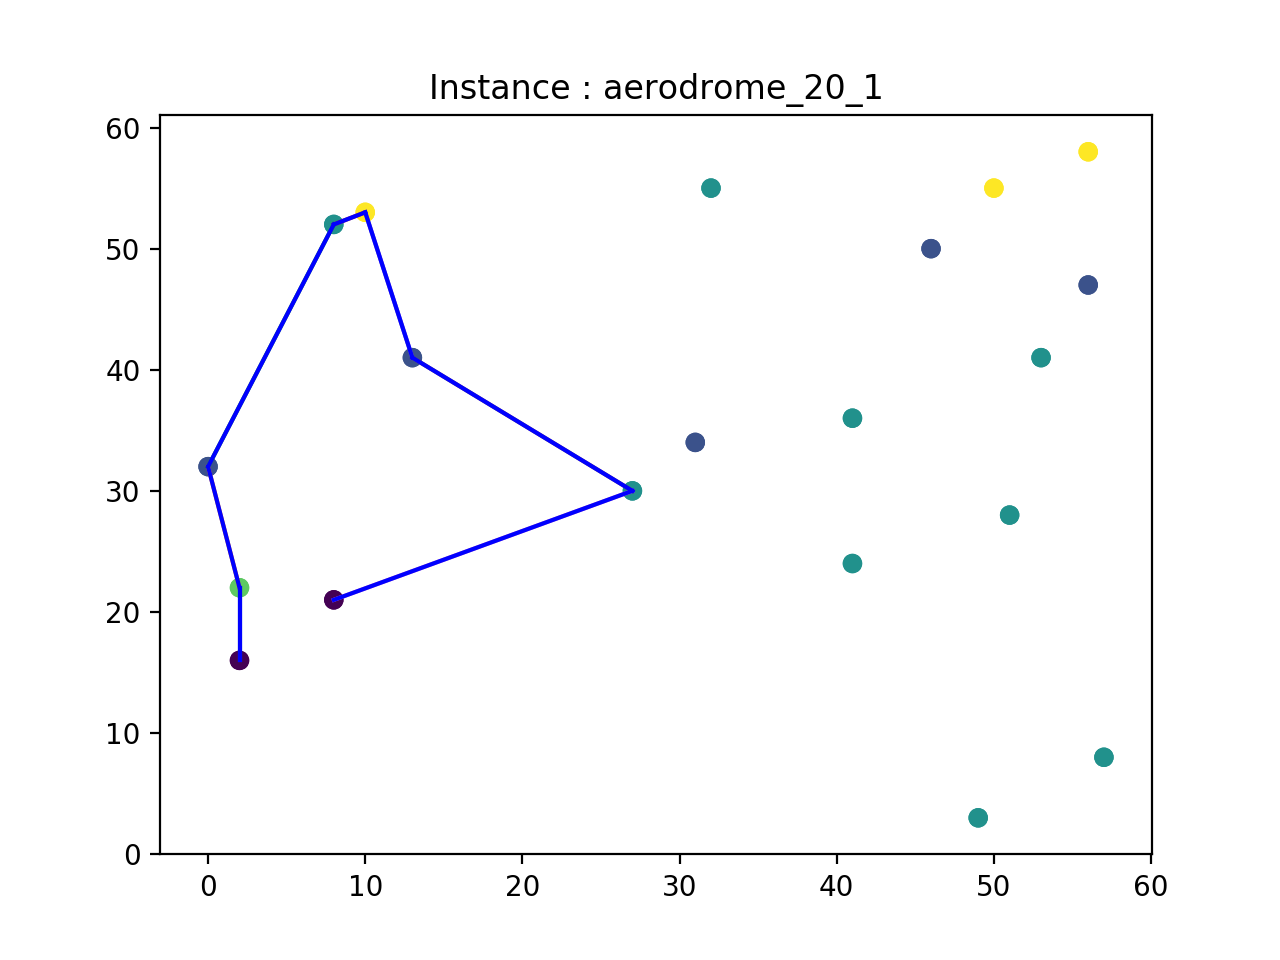
\includegraphics[scale=0.7]{20.png}
    \caption{Visualisation de la solution pour 20 aérodromes}
    \label{fig:20}
\end{figure}

\begin{figure}[!ht]
    \centering
    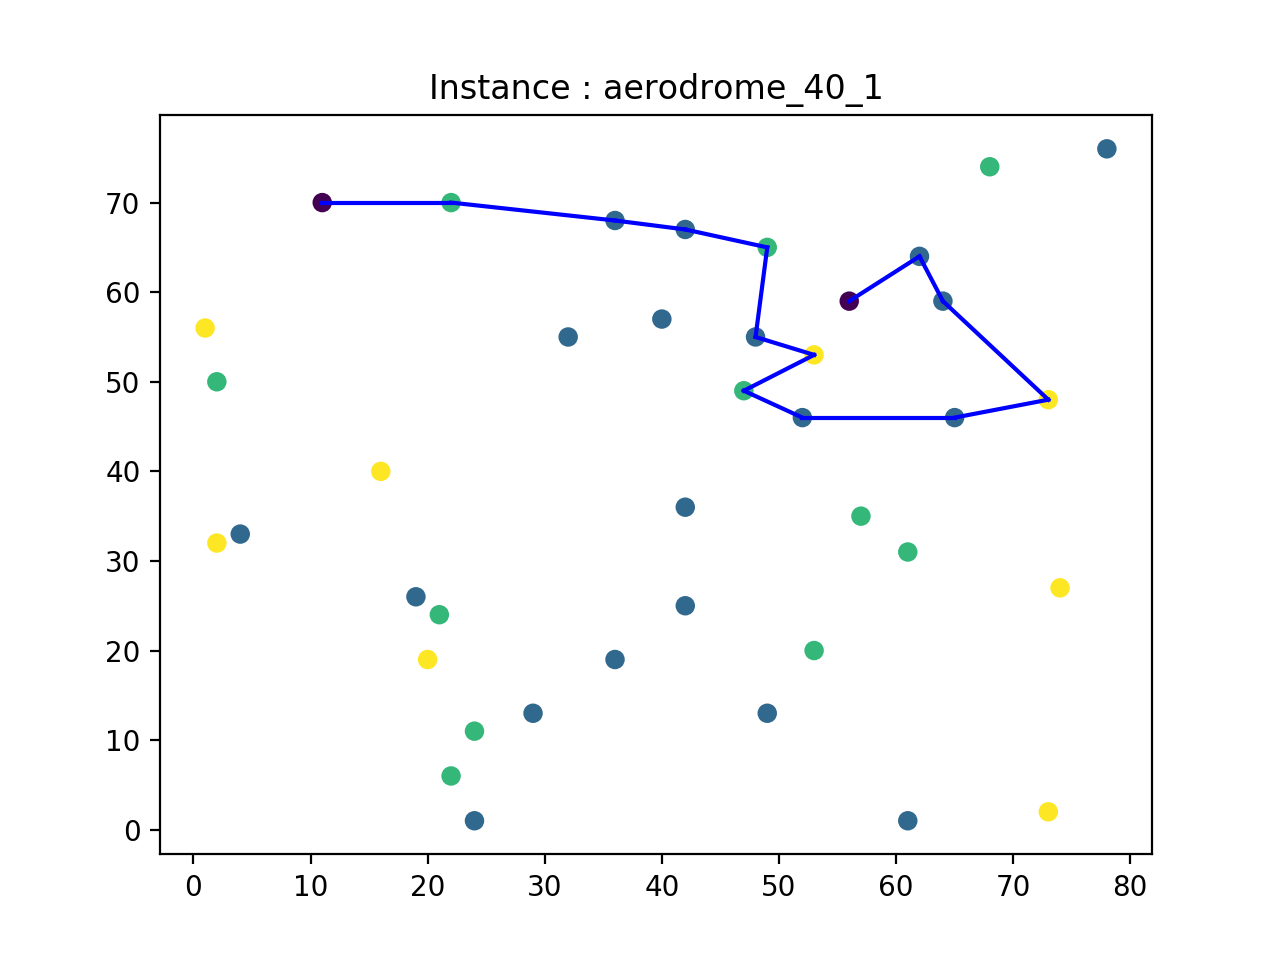
\includegraphics[scale=0.7]{40.png}
    \caption{Visualisation de la solution pour 40 aérodromes}
    \label{fig:20}
\end{figure}

\end{document}
